\documentclass[border=4pt]{standalone}
\usepackage{tikz}
\usetikzlibrary{arrows.meta}

\definecolor{orangeText}{HTML}{E3A063}
\definecolor{orangeDim}{HTML}{A87A4E}
\begin{document}
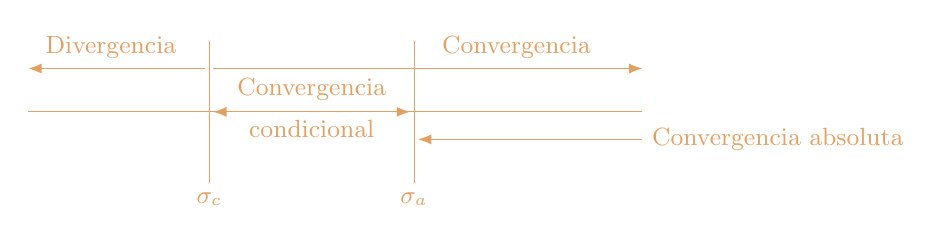
\begin{tikzpicture}[color=orangeText, >=Latex, x=1cm, y=1cm]

    % real line
    \draw (-3.6,0) -- (4.2,0);

    % abscissae of convergence
    \draw (-1.3,-0.9) -- (-1.3,0.9);
    \draw (1.3,-0.9) -- (1.3,0.9);
    \node[below] at (-1.3,-0.9) {\small $\sigma_c$};
    \node[below] at (1.3,-0.9) {\small $\sigma_a$};

    % divergence (left)
    \draw[<-] (-3.6,0.55) -- (-1.35,0.55);
    \node[above] at (-2.55,0.55) {\small Divergencia};

    % convergence (right)
    \draw[->] (-1.25,0.55) -- (4.2,0.55);
    \node[above] at (2.6,0.55) {\small Convergencia};

    % conditional convergence
    \draw[<->] (-1.25,0) -- (1.25,0);
    \node[above] at (0,0.02) {\small Convergencia};
    \node[below] at (0,0.02) {\small condicional};

    % absolute convergence
    \draw[<-] (1.35,-0.35) -- (4.2,-0.35);
    \node[right] at (4.2,-0.35) {\small Convergencia absoluta};

\end{tikzpicture}
\end{document}
